\documentclass[11pt,a4paper]{article}

\usepackage{fontspec}
\usepackage[margin=2.2cm]{geometry}
\usepackage{graphicx}
\usepackage{pdflscape}
\usepackage{longtable}
\usepackage{array}
\usepackage{booktabs}
\usepackage[table]{xcolor}
\usepackage{enumitem}
\usepackage{titlesec}
\usepackage{fancyhdr}
\usepackage[strings]{underscore}
\usepackage{hyperref}
\usepackage{caption}

\setmainfont{Georgia}

\definecolor{copetranblue}{HTML}{1D4ED8}
\definecolor{tablehead}{HTML}{EFF6FF}

\hypersetup{
  colorlinks=true,
  linkcolor=black,
  urlcolor=copetranblue,
  citecolor=black,
  pdftitle={Parcial Primer Corte - Diseño de Interfaz de Usuario - Copetran},
  pdfauthor={Santiago José Rodríguez Gutiérrez, Nicolás Pérez Chuscano, Camilo Andrés Díaz García}
}

\titleformat{\section}{\Large\bfseries\color{black}}{\thesection.}{0.5em}{}
\titleformat{\subsection}{\large\bfseries}{\thesubsection}{0.5em}{}

\pagestyle{fancy}
\setlength{\headheight}{14pt}
\fancyhf{}
\fancyhead[L]{Copetran --- Parcial Primer Corte}
\fancyhead[R]{\thepage}
\renewcommand{\headrulewidth}{0.4pt}

\newcolumntype{L}[1]{>{\raggedright\arraybackslash}p{#1}}

\begin{document}

% ---------------------------------------------------------------------------
% PORTADA
% ---------------------------------------------------------------------------
\begin{titlepage}
  \centering
  \vspace*{2cm}
  {\Large Universidad Sergio Arboleda\par}
  \vspace{0.3cm}
  {\large Facultad de Sistemas e Ingeniería\par}
  \vspace{2cm}

  {\huge\bfseries Parcial Primer Corte\par}
  \vspace{0.5cm}
  {\Large Diseño de la Interfaz de Usuario\par}
  \vspace{0.3cm}
  {\large Caso: Empresa Transportadora de Pasajeros a Nivel Nacional\\ con Servicios de Mensajería y Paquetes --- Copetran\par}

  \vspace{2.5cm}
  {\large\bfseries Integrantes\par}
  \vspace{0.3cm}
  {\large
    Santiago José Rodríguez Gutiérrez\\
    Nicolás Pérez Chuscano\\
    Camilo Andrés Díaz García\par
  }

  \vspace{2.5cm}
  {\large Patrones de Diseño de Software (SIST0076-G02)\\
  Docente: José Marcial Téllez Gómez\par}

  \vspace{1.5cm}
  {\large 7 de septiembre de 2026\par}

  \vfill
  {\small Repositorio de trabajo: \url{https://github.com/SKing25/Copetran-}\par}
\end{titlepage}

\tableofcontents
\newpage

% ---------------------------------------------------------------------------
\section{Introducción}
% ---------------------------------------------------------------------------

Este informe consolida el entregable \textbf{Parcial Primer Corte} del curso Patrones de Diseño
de Software, continuando el proyecto elegido: una \textbf{empresa transportadora de pasajeros a
nivel nacional con servicios de mensajería y paquetes} (Copetran). El entregable es distinto del
CR-1 T-2 (Formulación de Proyecto) ya presentado, pero se construye \textbf{100\% sobre él} ---
sobre el organigrama definitivo, el modelo relacional corregido en Microsoft SQL Server
(\texttt{copetran_corregido.sql}) y los procesos identificados con su rol responsable --- para
garantizar trazabilidad total entre ambos entregables. No se inventan roles, estados ni campos que
no estén ya documentados en esas fuentes.

La consigna de este parcial exige nueve componentes, que se documentan en las secciones
siguientes en el mismo orden en que fueron solicitados:

\begin{enumerate}[nosep]
  \item Definir roles del sistema.
  \item Casos de uso de alto nivel.
  \item Elegir dos procesos principales.
  \item Realizar dos casos de uso extendidos.
  \item Realizar dos formatos de especificación de caso de uso.
  \item Diagrama de clases DAO.
  \item Diagrama de estados para tres clases principales.
  \item Diagramas de colaboración para los dos procesos.
  \item Diagramas de secuencia para los dos procesos.
\end{enumerate}

Toda la documentación fuente de este informe reside en el repositorio de trabajo, bajo
\texttt{docs/parcial-primer-corte/}, organizada en un archivo por componente para facilitar su
revisión independiente.

% ---------------------------------------------------------------------------
\section{Roles del Sistema}
% ---------------------------------------------------------------------------

Los roles se extrajeron del organigrama definitivo de Copetran (CR-1 T-2, Sección 4), consolidando
los 22 grupos de cargo documentados en los que efectivamente operan pantallas o son actores de
caso de uso --- coherente con el requerimiento no funcional RNF01 (control de acceso por cargo).

\subsection{Actores primarios}

\begin{longtable}{L{3.6cm} L{4.6cm} L{6.5cm}}
\toprule
\rowcolor{tablehead}\textbf{Rol / Actor} & \textbf{Ubicación en el organigrama} & \textbf{Interviene en} \\
\midrule
\endhead
Cajero de Agencia & Dirección de Operaciones y Pasajes --- Comercial y Taquillas & Venta de tiquetes (A), reprogramación (G), registro de cliente (M) \\
Auxiliar de Despacho & Dirección de Operaciones y Pasajes --- Rodamiento y Despacho & Control de abordaje, cierre de tiquete VIAJADO/CANCELADO (A, B) \\
Operario de Bodega & Dirección de Logística y Carga --- Gestión de Bodegas y Hubs & Admisión y consolidación de mensajería (C), registro de cliente (M) \\
Conductor de Vehículo de Reparto & Dirección de Logística y Carga --- Distribución y Rutas de Carga & Distribución de última milla (H) \\
Analista de RRHH & Dirección de RRHH y Nómina --- Contratos y Licencias & Contratación (E) \\
Área de Nómina y Novedades & Dirección de RRHH y Nómina & Liquidación de nómina (E) \\
Técnico Mecánico & Dirección de Operaciones y Pasajes --- Mantenimiento de Flota & Mantenimiento y alta de flota (D, F) \\
Inspector Técnico / Auxiliar de Laboratorio & Dirección de Operaciones y Pasajes --- Seguridad Vial y Control & Alistamiento preoperacional (B) \\
Monitorista de Telemetría & Dirección de Tecnología TIC --- Centro de Control GPS e IoT & Monitoreo GPS/IoT (J) \\
Técnico de Incidencias (Mesa de Ayuda) & Dirección de Tecnología TIC & Gestión de incidencias TIC (I) \\
Administrador de Servidores & Dirección de Tecnología TIC --- Infraestructura y Ciberseguridad & Infraestructura y ciberseguridad (O) \\
Gerencia General / Direcciones & Transversal & Aprobación de rutas (K), gestión organizacional (L) \\
Auditoría Interna & Standalone, reporta a Gerencia & Verificación documental (B), trazabilidad (RNF06) \\
\bottomrule
\end{longtable}

\subsection{Actores secundarios / externos}

\begin{longtable}{L{5.5cm} L{2.8cm} L{6.4cm}}
\toprule
\rowcolor{tablehead}\textbf{Rol / Actor} & \textbf{Naturaleza} & \textbf{Interviene en} \\
\midrule
\endhead
Cliente (Pasajero / Remitente / Destinatario) & Externo, humano & Compra de tiquetes (A, canal WEB/APP), envío de mensajería (C) \\
Sistema de Pagos & Externo, sistema & Confirmación de pago (efectivo, débito, crédito, transferencia/QR) \\
Sistema de Facturación Electrónica (DIAN) & Externo, sistema & Emisión de CUFE (RF04, RNF07) \\
\bottomrule
\end{longtable}

% ---------------------------------------------------------------------------
\section{Casos de Uso de Alto Nivel}
% ---------------------------------------------------------------------------

Modelo de casos de uso de alto nivel UML V-2, organizado por rol, según la terminología del
docente (\emph{SEM 04 1 METODOLOGIAS RUP.pdf}):

\begin{itemize}[nosep]
  \item \textbf{Cliente:} Comprar Tiquete, Consultar Disponibilidad de Viaje, Reprogramar Tiquete Abierto, Cancelar Tiquete, Enviar Encomienda, Consultar Estado de Envío.
  \item \textbf{Cajero de Agencia:} Vender Tiquete, Emitir Factura, Reprogramar Tiquete, Registrar Cliente.
  \item \textbf{Auxiliar de Despacho:} Controlar Abordaje, Generar Planilla Única de Viaje, Cerrar Estado de Viaje.
  \item \textbf{Operario de Bodega:} Admitir Guía de Envío, Clasificar Mercancía, Consolidar Remesa, Actualizar Estado de Guía.
  \item \textbf{Conductor de Vehículo de Reparto:} Confirmar Entrega de Última Milla.
  \item \textbf{Analista de RRHH:} Registrar Empleado, Crear Contrato, Registrar Licencia de Conducción.
  \item \textbf{Área de Nómina y Novedades:} Registrar Novedad, Liquidar Nómina.
  \item \textbf{Técnico Mecánico:} Registrar Mantenimiento, Registrar Cambio de Placa, Dar de Alta un Bus.
  \item \textbf{Inspector Técnico / Auxiliar de Laboratorio:} Registrar Inspección Preoperacional, Registrar Prueba de Alcoholemia.
  \item \textbf{Monitorista de Telemetría:} Monitorear Dispositivo IoT, Generar Alerta de Desconexión.
  \item \textbf{Técnico de Incidencias:} Registrar Incidencia TIC, Cerrar Incidencia.
  \item \textbf{Administrador de Servidores:} Ejecutar Copia de Respaldo, Aplicar Parches de Seguridad.
  \item \textbf{Gerencia General:} Aprobar Apertura de Ruta/Agencia, Gestionar Estructura Organizacional.
  \item \textbf{Auditoría Interna:} Verificar Documentación de Vehículo/Conductor, Consultar Historial Auditable.
\end{itemize}

% ---------------------------------------------------------------------------
\section{Procesos Principales Elegidos}
% ---------------------------------------------------------------------------

Se eligieron el \textbf{Proceso A --- Venta de tiquetes de pasajeros} y el \textbf{Proceso C ---
Admisión y consolidación de mensajería en bodega} (numeración original del CR-1 T-2, Sección 5),
por las siguientes razones:

\begin{enumerate}
  \item Cubren las \textbf{dos líneas de negocio} de Copetran (pasajeros y carga/mensajería), no
  solo una --- el criterio de máxima cobertura pedido en la consigna.
  \item Son los \textbf{dos procesos con estados parametrizados más ricos} del modelo:
  \texttt{ESTADO_TIQUETE} (5 estados) y \texttt{ESTADO_GUIA} (5 estados), ideales para el diagrama
  de estados pedido.
  \item Ya están \textbf{documentados paso a paso con rol responsable} en el CR-1 T-2 (Secciones
  5.1 y 5.3), garantizando trazabilidad exacta entre este parcial y el entregable grande del
  curso.
  \item Tienen \textbf{requerimientos funcionales y hallazgos de auditoría ya trabajados} (RF03 y
  RF04 para el Proceso A; RF05, RF11 y RF17 para el Proceso C), lo que da contenido real para las
  reglas de negocio de las especificaciones de caso de uso.
\end{enumerate}

% ---------------------------------------------------------------------------
\section{Casos de Uso Extendidos}
% ---------------------------------------------------------------------------

\subsection{CUE-01 --- Comprar Tiquete de Pasajero (Proceso A)}

\begin{itemize}[nosep]
  \item \textbf{Actor principal:} Cajero de Agencia (canal TAQUILLA) / Cliente (canal WEB o APP).
  \item \textbf{Actores secundarios:} Sistema de Pagos, Auxiliar de Despacho.
  \item \texttt{<<include>>} \textbf{Consultar Disponibilidad de Silla} --- siempre se ejecuta antes de vender.
  \item \texttt{<<include>>} \textbf{Generar Factura} --- siempre se ejecuta al confirmar la venta.
  \item \texttt{<<extend>>} \textbf{Reservar Tiquete Sin Pago Inmediato} --- extiende el caso base cuando el cliente pide reserva temporal (estado \texttt{RESERVADO}, con \texttt{fecha_expiracion_reserva}).
  \item \texttt{<<extend>>} \textbf{Habilitar Tiquete Abierto} --- extiende el caso base cuando el pago se confirma pero el cliente pide viajar en fecha flexible (estado \texttt{ABIERTO}, con \texttt{penalidad_reprogramacion}).
  \item \texttt{<<extend>>} \textbf{Reprogramar Tiquete Abierto} (Proceso G) --- extiende cuando existe un tiquete en estado \texttt{ABIERTO} dentro de la fecha límite.
\end{itemize}

\subsection{CUE-02 --- Admitir y Consolidar Guía de Envío (Proceso C)}

\begin{itemize}[nosep]
  \item \textbf{Actor principal:} Operario de Bodega.
  \item \textbf{Actores secundarios:} Cliente (Remitente), Sistema de Facturación Electrónica.
  \item \texttt{<<include>>} \textbf{Clasificar Mercancía} --- siempre se ejecuta (categoría: general, perecedera, frágil, documentos/valores).
  \item \texttt{<<include>>} \textbf{Calcular Tarifa de Envío} --- siempre se ejecuta antes de generar la guía.
  \item \texttt{<<extend>>} \textbf{Asociar Guía a Factura Inmediata} --- extiende cuando el envío se paga en el momento de la admisión.
  \item \texttt{<<extend>>} \textbf{Consolidar en Remesa} --- extiende cuando la guía comparte remitente/destino con otras guías pendientes.
  \item \texttt{<<extend>>} \textbf{Marcar Guía con Novedad} --- extiende el flujo de seguimiento cuando el envío queda retenido (estado \texttt{NOVEDAD}).
\end{itemize}

% ---------------------------------------------------------------------------
\section{Especificación de Casos de Uso}
% ---------------------------------------------------------------------------

\subsection{ECU-01 --- Comprar Tiquete de Pasajero}

\begin{longtable}{L{3.2cm} L{11.3cm}}
\toprule
\textbf{ID} & ECU-01 \\
\textbf{Nombre} & Comprar Tiquete de Pasajero \\
\textbf{Actor(es)} & Cliente (principal en canal WEB/APP), Cajero de Agencia (principal en canal TAQUILLA), Sistema de Pagos (secundario) \\
\textbf{Descripción} & Permite registrar la venta de un tiquete para un viaje programado, bloqueando la silla seleccionada, generando la factura y confirmando el pago. \\
\textbf{Precondiciones} & Existe al menos un \texttt{VIAJE_PROGRAMADO} con sillas disponibles; el cliente está registrado o se registra en el paso 2 (Proceso M). \\
\textbf{Postcondiciones} & Se crea un \texttt{TIQUETE} en estado \texttt{PAGADO} (o \texttt{RESERVADO}/\texttt{ABIERTO} según flujo alterno) asociado a una \texttt{FACTURA}; la silla queda ocupada para ese viaje (\texttt{UNIQUE(id_viaje, id_silla)}, RF01). \\
\textbf{Flujo principal} &
\begin{enumerate}[nosep,leftmargin=*]
  \item Consultar disponibilidad de sillas del viaje.
  \item Seleccionar silla y registrar/reutilizar datos del cliente.
  \item Definir canal de venta (TAQUILLA, WEB, APP).
  \item Bloquear la silla temporalmente (RF03, p.\ ej.\ 3 minutos) para evitar condición de carrera entre canales.
  \item Emitir factura (cliente, cajero, método de pago).
  \item Confirmar recepción del pago.
  \item Confirmar tiquete como \texttt{PAGADO}.
\end{enumerate} \\
\textbf{Flujos alternativos} &
\textbf{A1 (Reserva sin pago inmediato):} en el paso 6 el cliente no paga de inmediato --- el tiquete queda en \texttt{RESERVADO} con \texttt{fecha_expiracion_reserva}; si vence sin pago, se libera la silla.\newline
\textbf{A2 (Tiquete abierto):} en el paso 7 el cliente solicita flexibilidad de fecha --- estado \texttt{ABIERTO} con \texttt{penalidad_reprogramacion}.\newline
\textbf{A3 (Cancelación):} el Auxiliar de Despacho marca el tiquete como \texttt{CANCELADO} si no se usa. \\
\textbf{Reglas de negocio} & RF03 (bloqueo temporal de silla, un tiquete por silla por viaje), RF04 (factura debe emitir CUFE), 5 estados y 3 canales parametrizados en \texttt{MULTITABLA_PARAMETRO}. \\
\textbf{Frecuencia de uso} & Alta --- varias veces por minuto en horas pico, por agencia. \\
\bottomrule
\end{longtable}

\subsection{ECU-02 --- Admitir y Consolidar Guía de Envío}

\begin{longtable}{L{3.2cm} L{11.3cm}}
\toprule
\textbf{ID} & ECU-02 \\
\textbf{Nombre} & Admitir y Consolidar Guía de Envío \\
\textbf{Actor(es)} & Operario de Bodega (principal), Cliente/Remitente (secundario), Sistema de Facturación (secundario) \\
\textbf{Descripción} & Permite admitir un paquete en bodega, clasificarlo, generar su guía con código de barras y, si aplica, consolidarlo en una remesa. \\
\textbf{Precondiciones} & El remitente y el destinatario están registrados o se registran en el momento (Proceso M). \\
\textbf{Postcondiciones} & Se crea una \texttt{GUIA_ENVIO} en estado \texttt{ADMITIDO}, con o sin \texttt{id_remesa} asociado; si se paga en el momento, queda asociada a una \texttt{FACTURA}. \\
\textbf{Flujo principal} &
\begin{enumerate}[nosep,leftmargin=*]
  \item Admisión: registrar remitente, destinatario, pesaje y dimensionamiento.
  \item Clasificar mercancía (general, perecedera, frágil, documentos/valores).
  \item Calcular tarifa y generar guía con código de barras (estado \texttt{ADMITIDO}).
  \item Recepción en bodega/hub, con control de capacidad/temperatura si aplica.
  \item Consolidar en remesa si comparte remitente/destino con otras guías pendientes.
  \item Actualizar estado a lo largo del ciclo: \texttt{EN_TRANSITO} $\rightarrow$ \texttt{BODEGA_DESTINO} $\rightarrow$ \texttt{ENTREGADO}.
\end{enumerate} \\
\textbf{Flujos alternativos} &
\textbf{A1 (Pago inmediato):} en el paso 3, si el envío se paga al momento, se asocia \texttt{id_factura}.\newline
\textbf{A2 (Envío sin remesa):} en el paso 5, una guía puede viajar sin consolidarse en remesa.\newline
\textbf{A3 (Novedad):} en cualquier punto del paso 6, el estado puede pasar a \texttt{NOVEDAD} si el envío queda retenido. \\
\textbf{Reglas de negocio} & RF05 (cálculo automático de valor según peso/categoría, seguimiento de estado), RF11 (hallazgo: el modelo aún no registra qué empleado ejecuta la admisión --- pendiente de corrección), RF17 (los totales de la remesa deben recalcularse a partir de sus guías --- pendiente de trigger, ver auditoría CR-1 T-2 Sección 14.6). \\
\textbf{Frecuencia de uso} & Alta --- continua durante horario operativo, por bodega/hub. \\
\bottomrule
\end{longtable}

% ---------------------------------------------------------------------------
\section{Diagrama de Clases DAO}
% ---------------------------------------------------------------------------

El diagrama organiza las clases en dos paquetes --- \textbf{Capa de Acceso a Datos (DAO)} y
\textbf{Capa de Entidades (Modelo de Dominio)} --- sin flechas cruzando entre capas: la relación
entre cada clase \texttt{*DAO} y su entidad homónima se identifica por nombre y por la posición
equivalente en ambos paquetes. \texttt{ConexionBD} implementa el patrón \emph{Singleton} (GoF) y
es la única fuente de conexión para todas las clases DAO, que a su vez implementan la interfaz
genérica \texttt{GenericDAO<T>}.

\begin{landscape}
\begin{figure}[p]
  \centering
  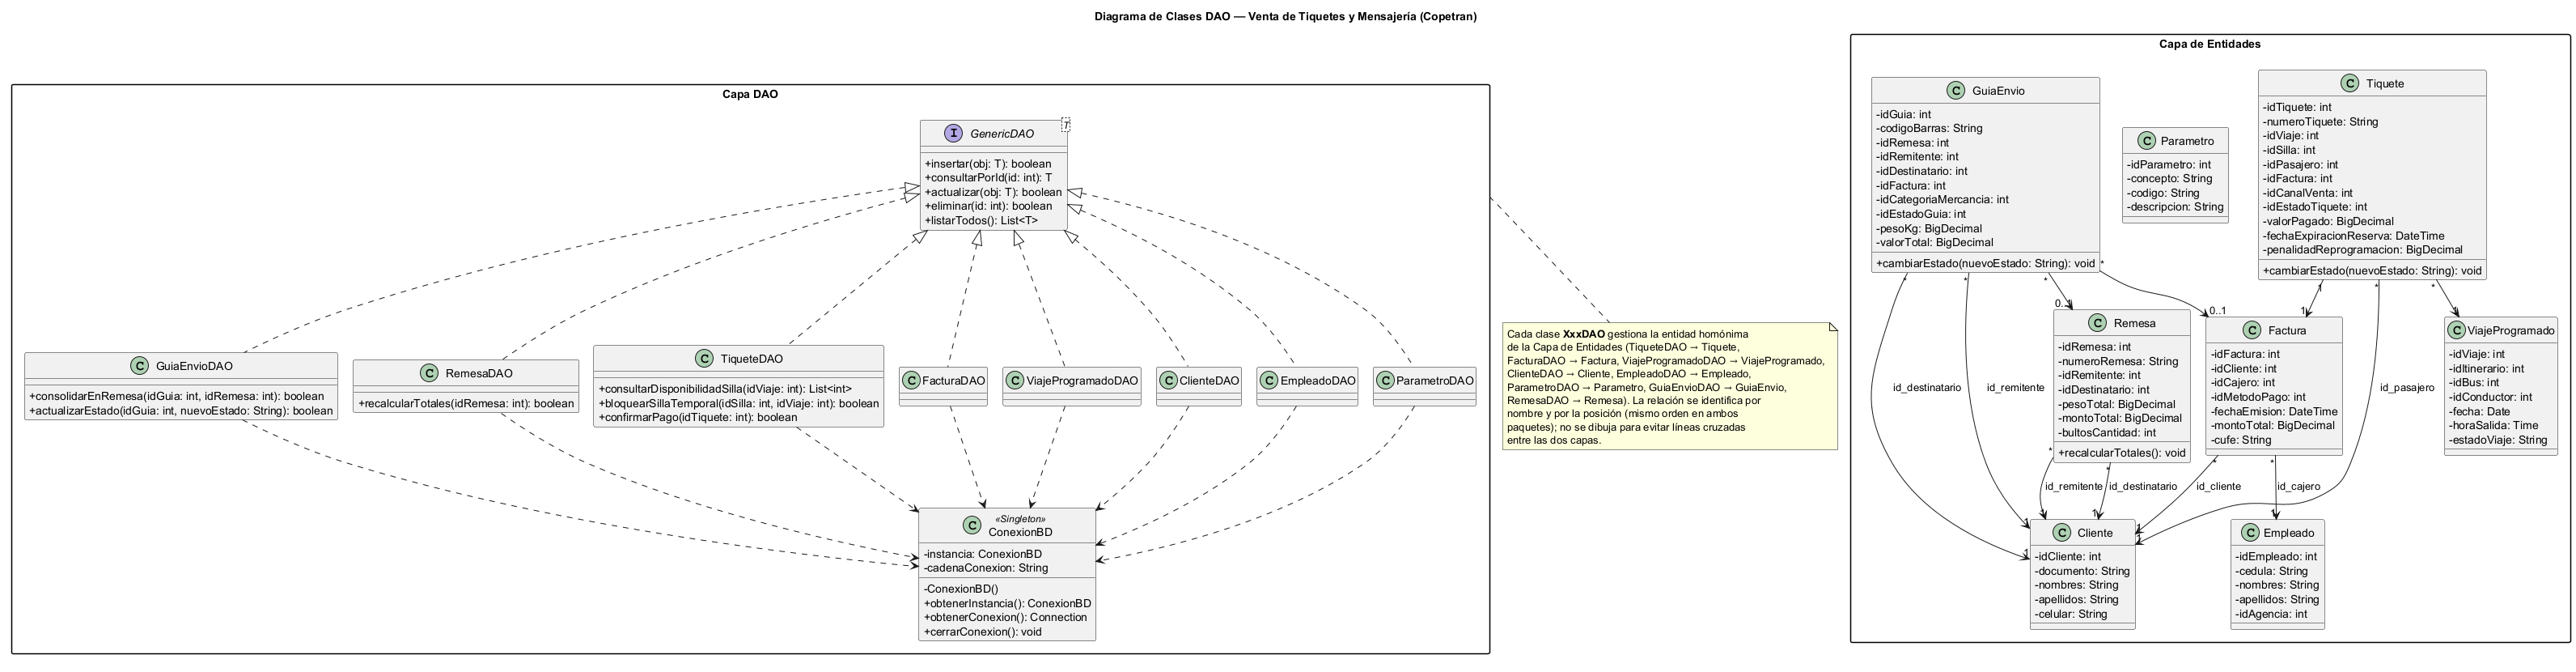
\includegraphics[width=\linewidth]{diagramas/clases-dao/clases_dao.png}
  \caption{Diagrama de clases DAO --- Venta de Tiquetes y Mensajería (Copetran)}
\end{figure}
\end{landscape}

% ---------------------------------------------------------------------------
\section{Diagramas de Estados}
% ---------------------------------------------------------------------------

Se modelan los tres estados/ciclos de vida más ricos del sistema, correspondientes a las clases
\texttt{Tiquete}, \texttt{GuiaEnvio} y \texttt{ViajeProgramado}.

\subsection{Clase \texttt{Tiquete} (\texttt{ESTADO_TIQUETE})}

\begin{figure}[h!]
  \centering
  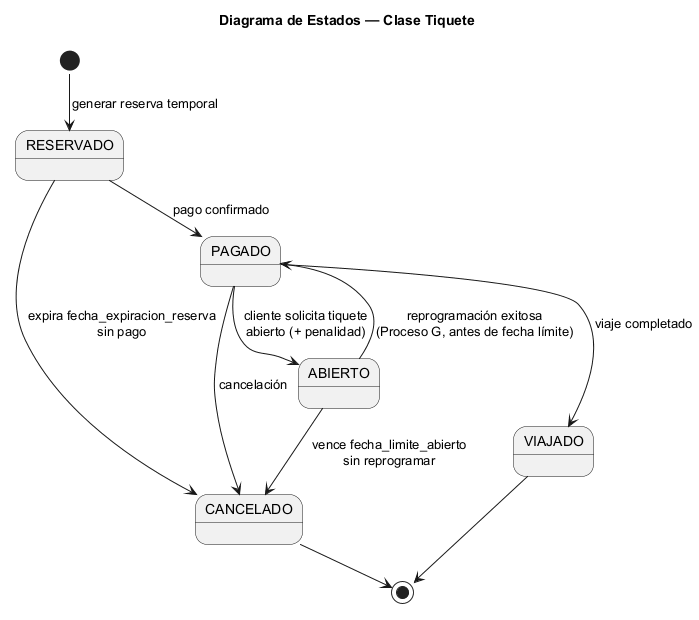
\includegraphics[width=0.7\linewidth]{diagramas/estados/estado_tiquete.png}
  \caption{Diagrama de estados --- Clase Tiquete}
\end{figure}

\clearpage
\subsection{Clase \texttt{GuiaEnvio} (\texttt{ESTADO_GUIA})}

\begin{figure}[h!]
  \centering
  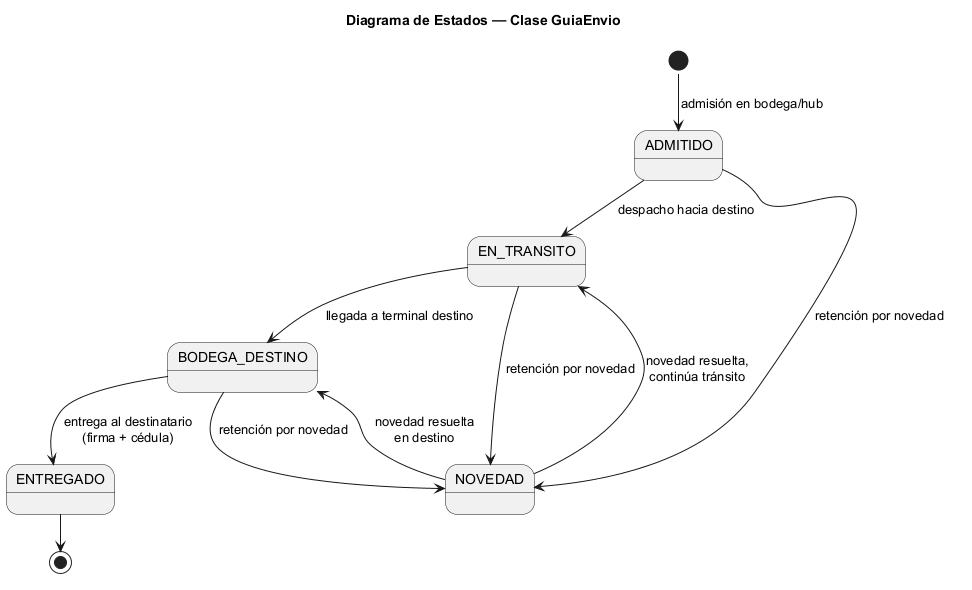
\includegraphics[width=0.85\linewidth]{diagramas/estados/estado_guia_envio.png}
  \caption{Diagrama de estados --- Clase GuiaEnvio}
\end{figure}

\subsection{Clase \texttt{ViajeProgramado} (\texttt{estado_viaje})}

\emph{Nota:} en el modelo relacional actual \texttt{estado_viaje} es texto libre (hallazgo de
normalización, CR-1 T-2 Sección 14.6). Este diagrama formaliza el comportamiento real descrito en
el Proceso B, y sirve como insumo para migrar el campo a \texttt{MULTITABLA_PARAMETRO} en una
futura iteración.

\begin{figure}[h!]
  \centering
  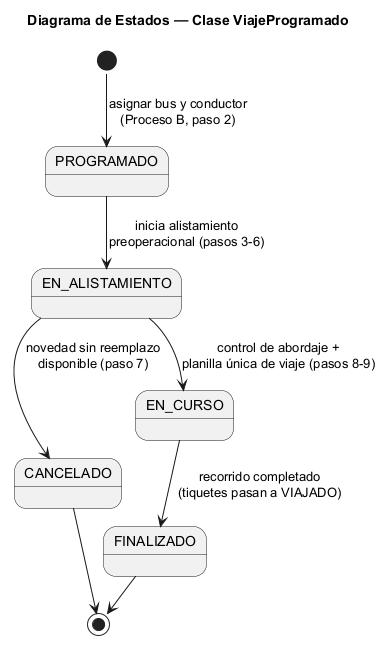
\includegraphics[width=0.5\linewidth]{diagramas/estados/estado_viaje_programado.png}
  \caption{Diagrama de estados --- Clase ViajeProgramado}
\end{figure}

\clearpage
% ---------------------------------------------------------------------------
\section{Diagramas de Colaboración}
% ---------------------------------------------------------------------------

PlantUML no tiene un tipo nativo ``diagrama de comunicación/colaboración''; se representa como
diagrama de objetos con mensajes numerados sobre los enlaces (técnica estándar UML2 para
aproximar un diagrama de colaboración).

\subsection{Proceso A --- Venta de Tiquetes}

\begin{figure}[h!]
  \centering
  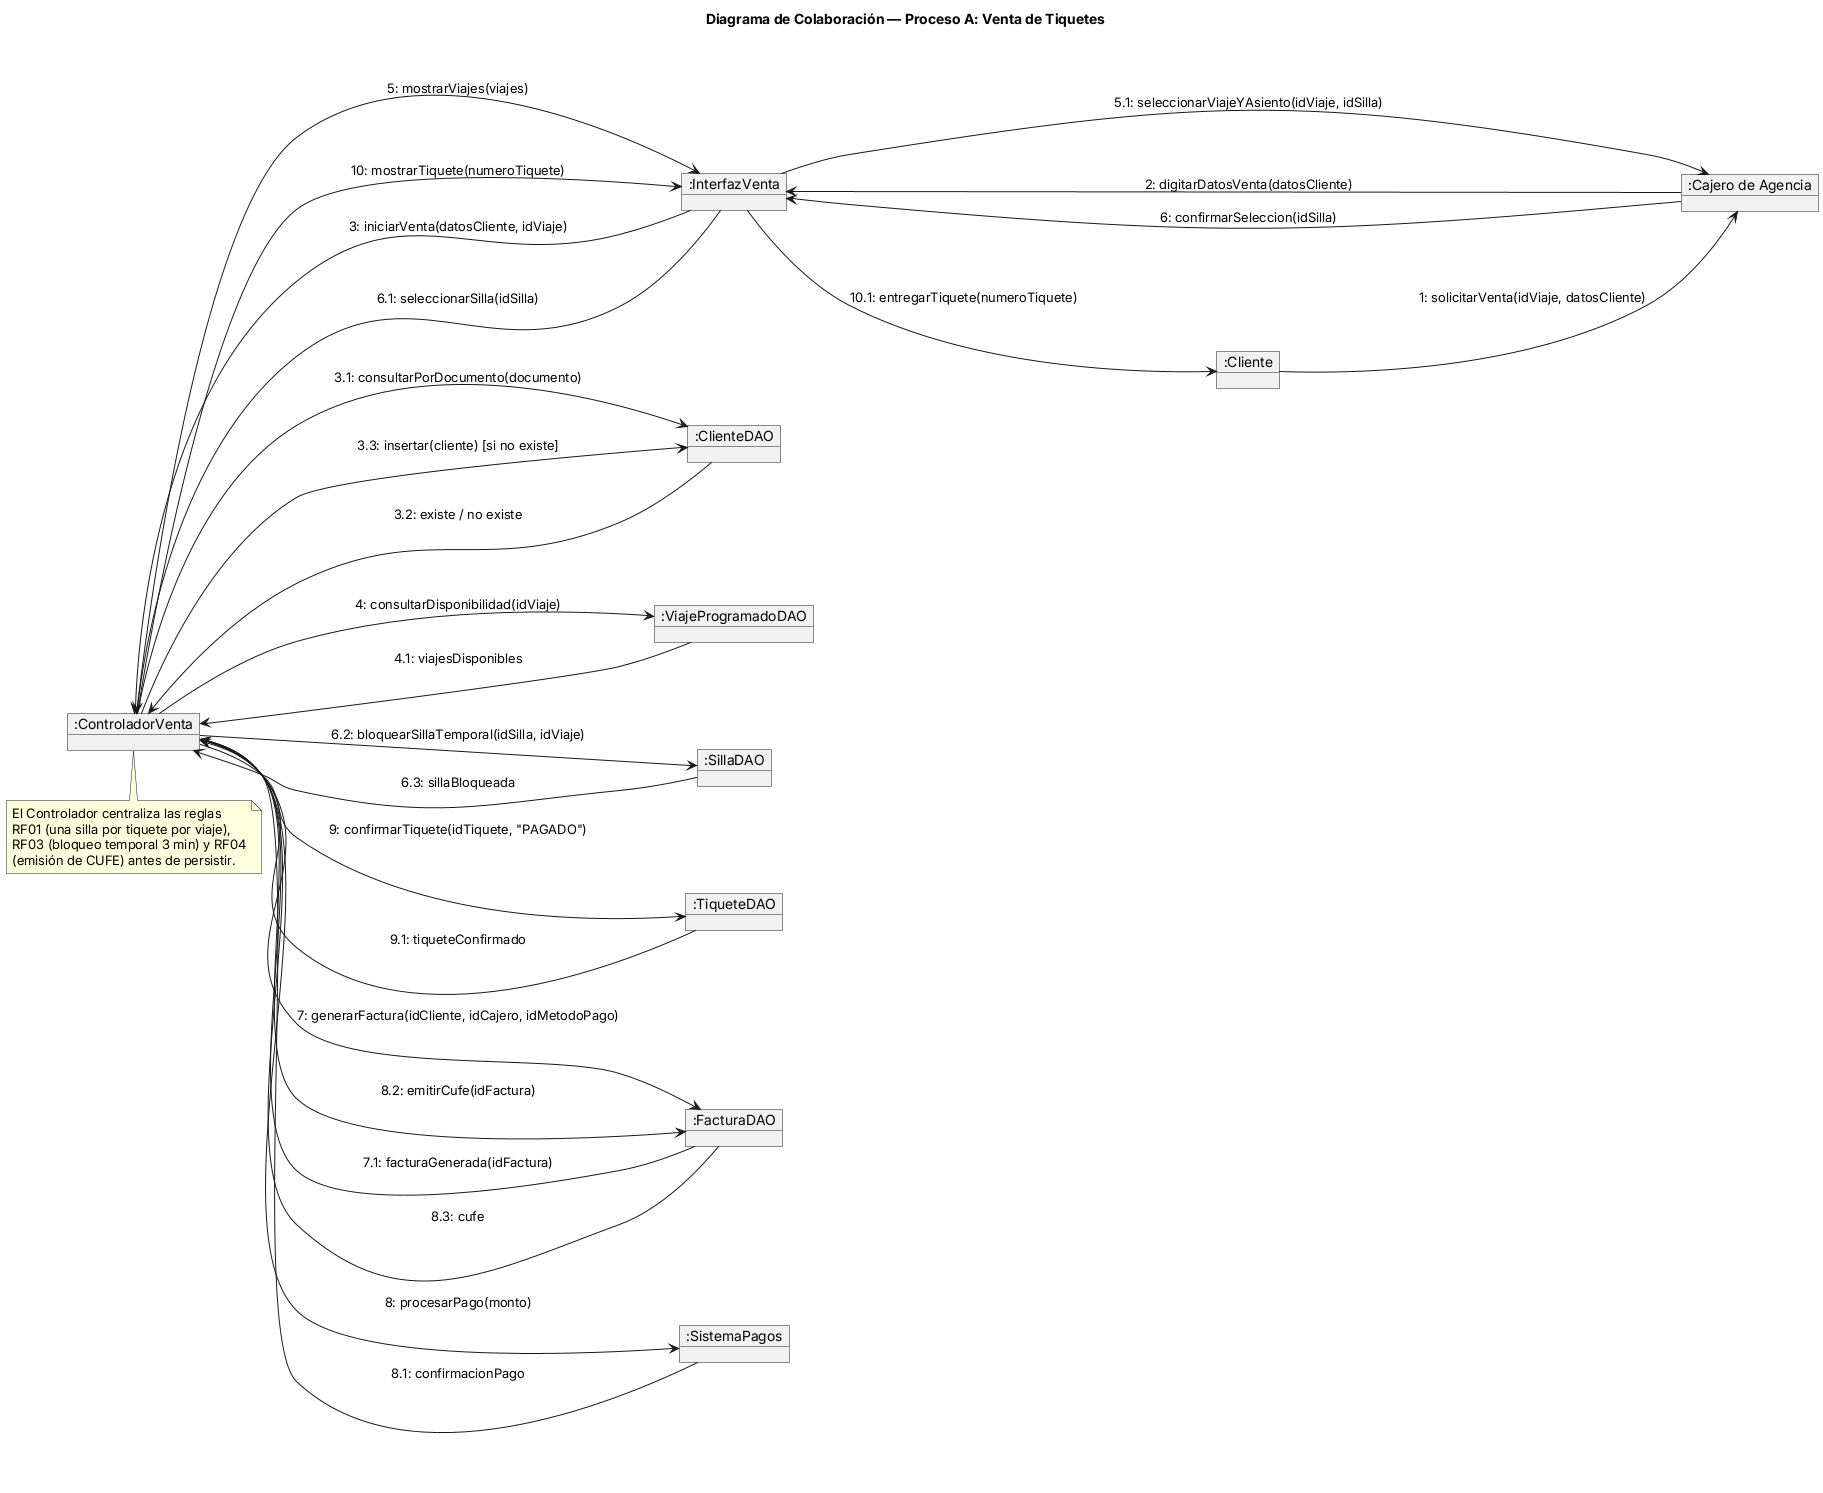
\includegraphics[width=\linewidth]{diagramas/colaboracion/colaboracion_venta_tiquetes.png}
  \caption{Diagrama de colaboración --- Proceso A: Venta de Tiquetes}
\end{figure}

\subsection{Proceso C --- Admisión y Consolidación de Mensajería}

\begin{figure}[h!]
  \centering
  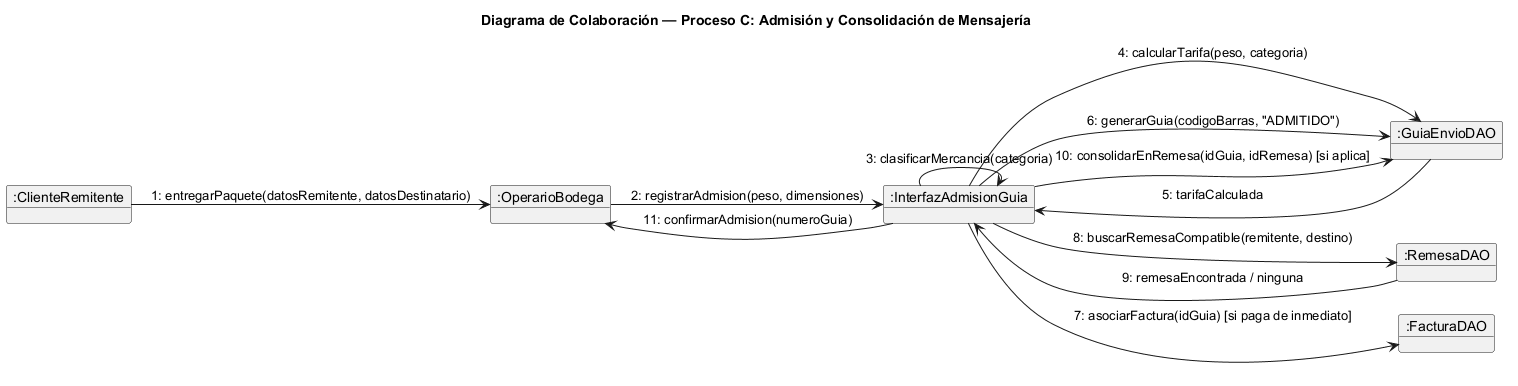
\includegraphics[width=\linewidth]{diagramas/colaboracion/colaboracion_admision_mensajeria.png}
  \caption{Diagrama de colaboración --- Proceso C: Admisión y Consolidación de Mensajería}
\end{figure}

\clearpage
% ---------------------------------------------------------------------------
\section{Diagramas de Secuencia}
% ---------------------------------------------------------------------------

\subsection{Proceso A --- Venta de Tiquetes}

\begin{figure}[h!]
  \centering
  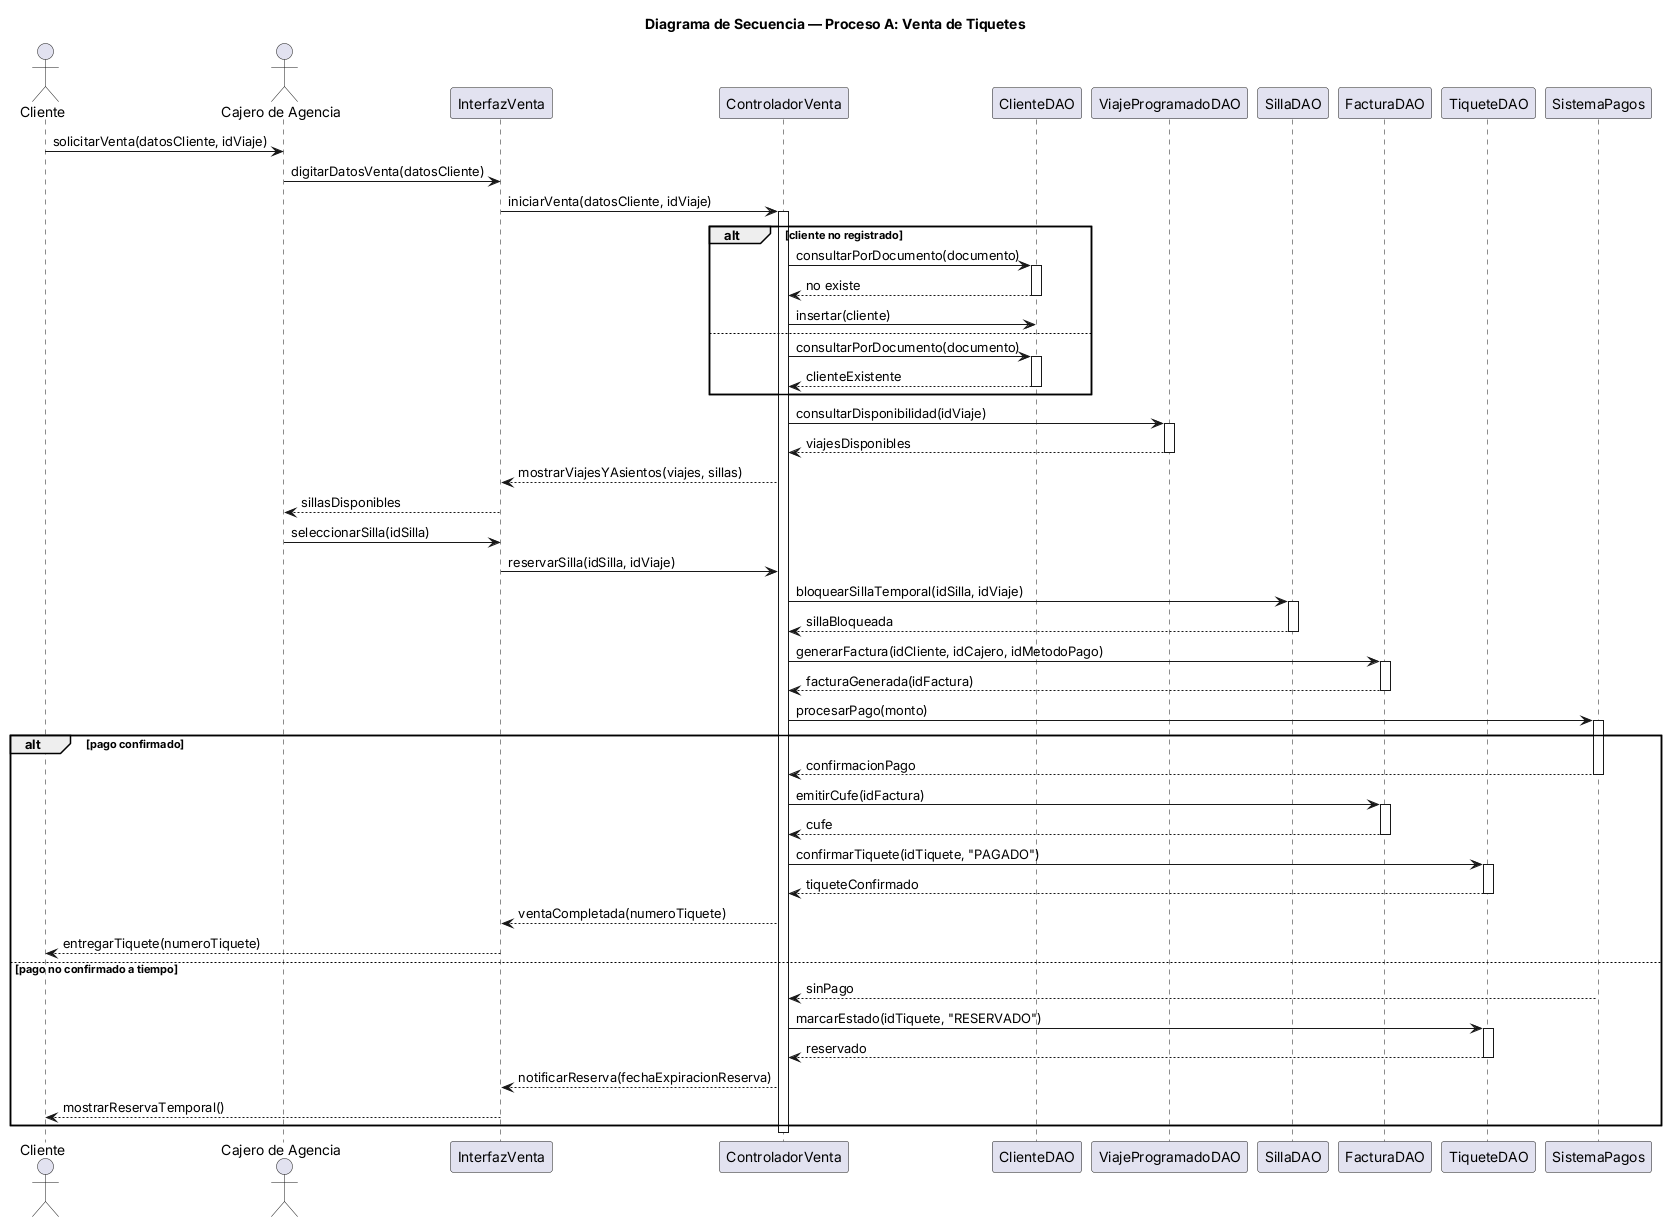
\includegraphics[width=0.95\linewidth]{diagramas/secuencia/secuencia_venta_tiquetes.png}
  \caption{Diagrama de secuencia --- Proceso A: Venta de Tiquetes}
\end{figure}

\clearpage
\subsection{Proceso C --- Admisión y Consolidación de Mensajería}

\begin{figure}[h!]
  \centering
  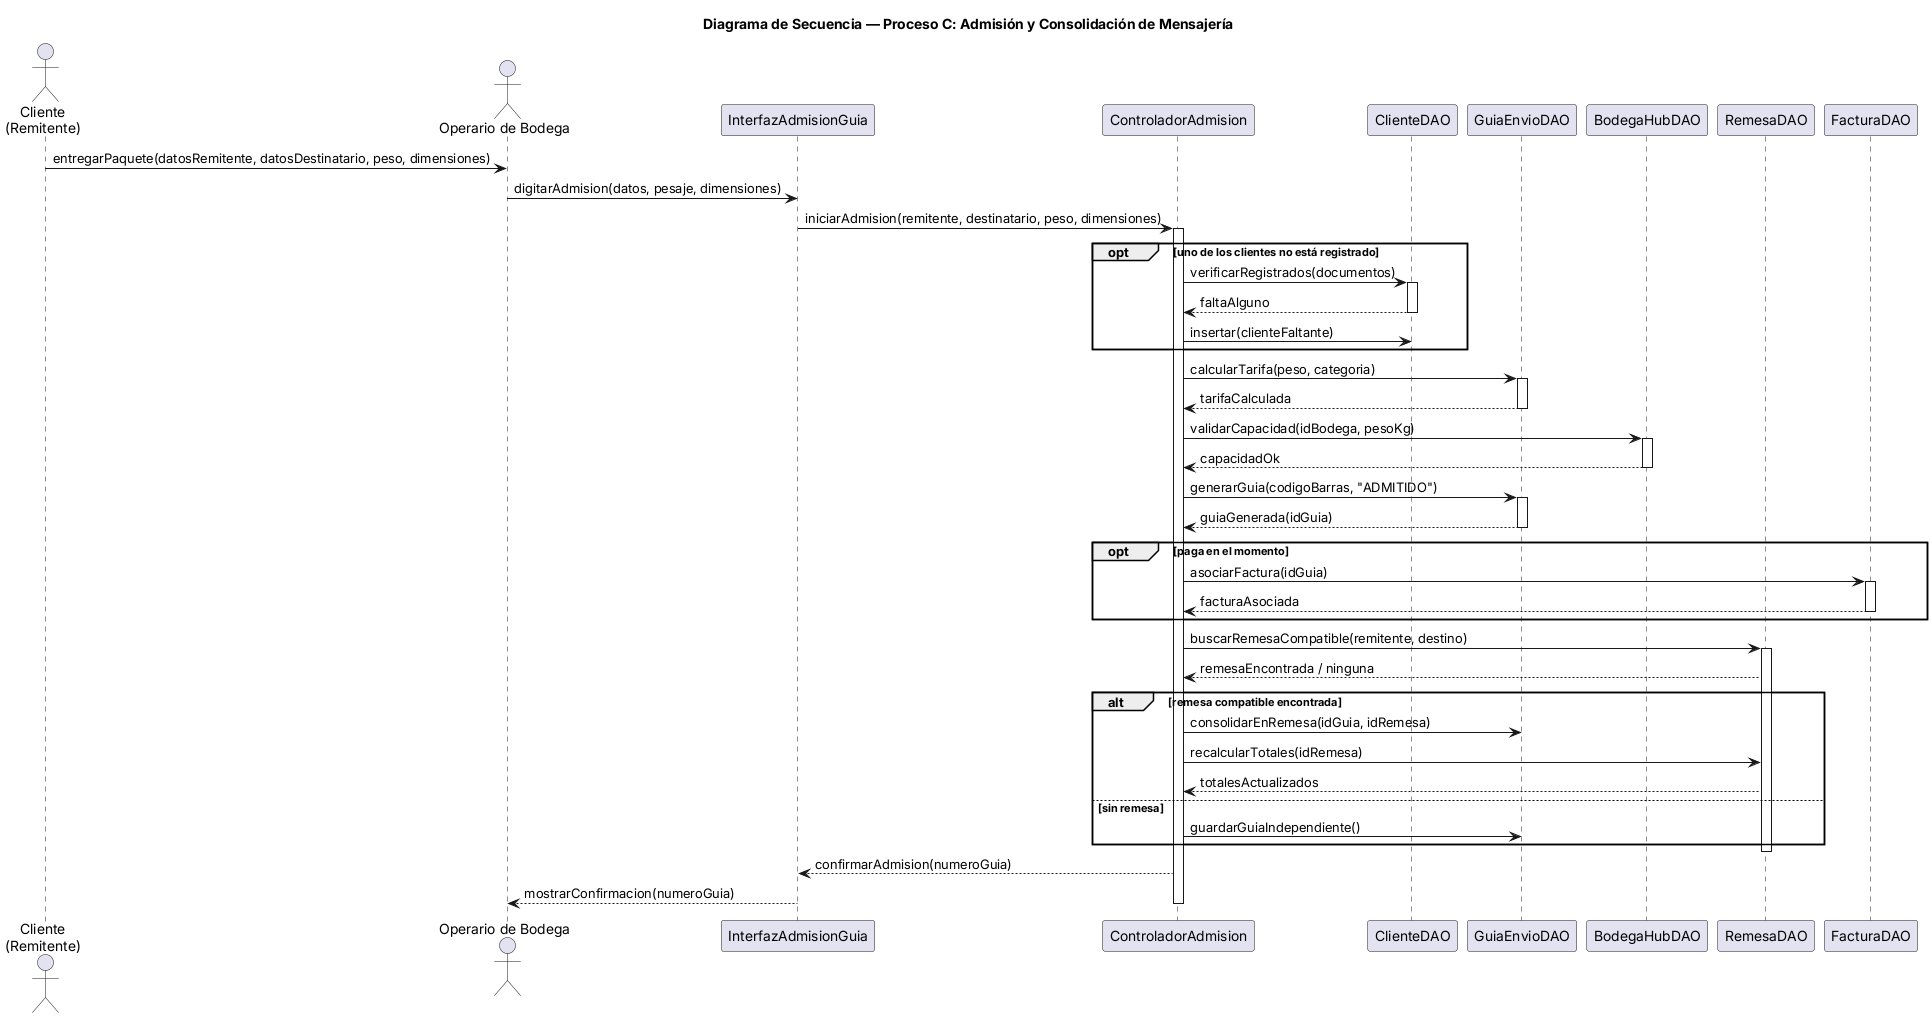
\includegraphics[width=0.95\linewidth]{diagramas/secuencia/secuencia_admision_mensajeria.png}
  \caption{Diagrama de secuencia --- Proceso C: Admisión y Consolidación de Mensajería}
\end{figure}

\clearpage
% ---------------------------------------------------------------------------
\section{Notas de Trazabilidad y Pendientes}
% ---------------------------------------------------------------------------

\begin{itemize}
  \item El diagrama de estados de \texttt{ViajeProgramado} formaliza un campo que hoy es texto
  libre en la base de datos (hallazgo de normalización, CR-1 T-2 Sección 14.6) --- se documenta
  explícitamente como aporte de este parcial.
  \item ECU-02 hereda el hallazgo RF11 (falta \texttt{id_empleado} en \texttt{GUIA_ENVIO}) y RF17
  (falta trigger de recálculo de totales en \texttt{REMESA}) --- el diagrama de clases DAO ya
  incluye \texttt{recalcularTotales()} como método propuesto en \texttt{RemesaDAO}/\texttt{Remesa},
  coherente con la corrección pendiente documentada en el CR-1 T-2.
  \item Este documento y sus diagramas son un entregable \textbf{aparte} del CR-1 T-2
  (\path{cr1_t2_formulacion_proyecto.tex}); no lo reemplazan ni se fusionan con ese archivo salvo
  que el equipo decida lo contrario más adelante.
  \item Como complemento --- fuera del alcance estricto de esta consigna --- el equipo desarrolló
  también un escafolding funcional de la interfaz de usuario (React + TypeScript + Vite +
  TailwindCSS) en la carpeta \texttt{frontend/} del repositorio, implementando ECU-01 y ECU-02
  sobre datos de prueba en memoria, disponible para demostración en la sustentación.
\end{itemize}

\end{document}
